\documentclass{beamer}
\usepackage{amsmath, graphicx}
\usepackage{verbatim}
\usetheme{Madrid}
\usepackage{listings}
\usepackage{tikz}

\usepackage{listings}
\lstset{language=C}



\title{Somatórios e Computação Numérica}
\author{Professores Claudia Tavares e Luiz Otávio Rodrigues Alves Sereno}
\date{Curso: Ciência da Computação}

\begin{document}

\begin{frame}
    \titlepage
    \vfill
    \begin{center}
    \vspace{-0.9cm}
        \includegraphics[width=0.25\textwidth]{logopuc.png} \hspace{1.4cm}
        \includegraphics[width=0.25\textwidth]{logoicei.jpg}
    \end{center}
\end{frame}

\begin{frame}{Algoritmos Iterativos}
    
   \begin{block}{Algoritmos iterativos}
Um algoritmo iterativo refere-se a um procedimento matemático usado para resolver problemas, aproximando resultados com base em respostas obtidas anteriormente. 
    \end{block} 
\end{frame}

\begin{frame}{Somatórios}
    O operador de somatório é uma notação conveniente para representar somas de uma sequência de termos:
    \[
        \sum_{k=1}^{n} a_k = a_1 + a_2 + \dots + a_n.
    \]
    O somatório é amplamente utilizado no Cálculo para descrever somas finitas e infinitas, sendo essencial em diversos métodos numéricos e integrais aproximadas.
\end{frame}

\begin{frame}{Propriedades dos Somatórios}
    Algumas propriedades úteis do operador de somatório incluem:
    \begin{itemize}
    \item Soma de constante: \( \displaystyle \sum_{k=1}^{n} 1 = n\)
        \item Fatoração de constantes: \( \displaystyle \sum_{k=1}^{n} c a_k = c \sum_{k=1}^{n} a_k \)
        \item Linearidade: \( \displaystyle \sum_{k=1}^{n} (a_k + b_k) = \sum_{k=1}^{n} a_k + \sum_{k=1}^{n} b_k \)
        \item Soma de uma progressão aritmética: \( \displaystyle \sum_{k=1}^{n} k = \frac{n(n+1)}{2} \)
        \item Soma de uma progressão geométrica: \( \displaystyle \sum_{k=0}^{n} r^k = \frac{1 - r^{n+1}}{1 - r}, \quad r \neq 1 \)
    \end{itemize}
\end{frame}


\begin{frame}{Computação Numérica}
    Computação numérica é um campo de estudo que usa técnicas computacionais e analíticas para resolver problemas matemáticos de forma aproximada. 
\end{frame}

\begin{frame}{Computação Numérica - Exemplos}
    \begin{itemize}
        \item Soma de Riemann e Integrais Definidas
        \item Regra dos Trapézios e Integrais Definidas
        \item Séries numéricas e Aproximações
        \item Séries numéricas e funções
    \end{itemize}
\end{frame}


\begin{frame}{Soma de Riemann e Integrais Definidas}
    A soma de Riemann é uma aplicação fundamental do somatório para definir integrais definidas:
    \[
        \int_{a}^{b} f(x) dx = \lim_{n \to \infty} \sum_{i=1}^{n} f(x_i^*) \Delta x.
    \]
    Onde \( \Delta x = \displaystyle \frac{b-a}{n} \) representa a largura dos subintervalos e $x_i^*$ são pontos amostrais em cada um desses subintervalos.
\end{frame}

\begin{frame}{Exemplo: Soma de Riemann para \( f(x) = x^2 \)}
    Para aproximar \( \int_{0}^{1} x^2 dx \) usando a soma de Riemann com \( n=4 \):
    \begin{enumerate}
        \item Definimos \( \Delta x = \displaystyle \frac{1-0}{4} = 0.25 \).
        \item Escolhemos pontos médios: \( x_i = 0.125, 0.375, 0.625, 0.875 \).
        \item Calculamos \( \sum f(x_i) \Delta x \).
    \end{enumerate}

    \begin{figure}[h]
    \centering
    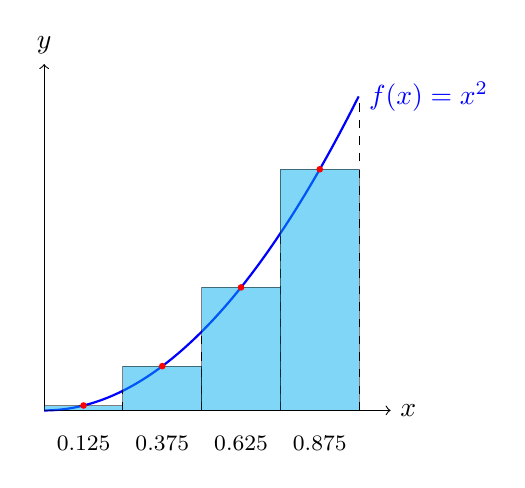
\begin{tikzpicture}[scale=4]
        % Eixos
        \draw[->] (0,0) -- (1.1,0) node[right] {$x$};
        \draw[->] (0,0) -- (0,1.1) node[above] {$y$};

        % Função f(x) = x^2
        \draw[domain=0:1, samples=100, thick, blue] plot (\x, {\x*\x}) node[right] {$f(x) = x^2$};

        % Subdivisão do intervalo [0,1] em 4 partes
        \foreach \x in {0,0.25,0.5,0.75,1} {
            \draw[dashed] (\x,0) -- (\x, {\x*\x});
        }

        % Pontos médios e retângulos
        \foreach \x in {0.125,0.375,0.625,0.875} {
            \draw[fill=cyan,opacity=0.5] (\x-0.125,0) rectangle (\x+0.125, {\x*\x});
            \fill[red] (\x, {\x*\x}) circle (0.3pt);
        }

        % Rótulos dos pontos médios
        \foreach \x in {0.125,0.375,0.625,0.875} {
            \draw (\x, -0.05) node[below] {\footnotesize $\x$};
        }
    \end{tikzpicture}
    \caption{Soma de Riemann com pontos médios para \( f(x) = x^2 \) e \( n=4 \).}
\end{figure}

\end{frame}

\begin{frame}{Atividade Prática 1:}
    Use uma soma de Riemann para aproximar \( \displaystyle \int_{1}^{11} (x^2 - 2x + 4) dx \) usando a soma de Riemann com \( n=5 \) e considerando o ponto médio de cada subintervalo.

\end{frame}

\begin{frame}{Regra dos Trapézios}

\begin{figure}
    \centering
    \includegraphics[width=8cm]{trapezios.jpg}
    \caption{Regra dos Trapézios}
    \label{fig:my_label}
\end{figure}

\end{frame}


\begin{frame}{Regra dos Trapézios}
    A Regra dos Trapézios utiliza somatórios para aproximar integrais:
    \[
        \int_{a}^{b} f(x) dx \approx 
        \frac{h}{2} [f(x_0)+2\sum_{i=1}^{n-1} f(x_i) + f(x_n)]
    \]
    onde \( h = \frac{b-a}{n} \) é a largura dos subintervalos.
\end{frame}


%------------------------------------------------------------
\begin{frame}{Regra dos Trapézios - Algoritmo}
Início

\hspace{0.5cm} $h \leftarrow (x_n - x_0) / n$

\hspace{0.5cm} $x \leftarrow x_0 + h$

\hspace{0.5cm} $soma \leftarrow 0$

\hspace{0.5cm} Para $i = 1$ até $n - 1$ Faça

\hspace{1.3cm} $soma \leftarrow soma + f(x)$

\hspace{1.3cm} $x \leftarrow x + h$

\hspace{0.5cm} $R \leftarrow \frac{h}{2} \left(f(x_0)  + 2soma + f(x_n) \right)$

Escreva(‘O resultado da integral da função $f$ é ’, $R$)

Fim
\end{frame}


\begin{frame}{Atividade Prática 2:}
    Considere a função \( f(x) = x^2 \) no intervalo \([0,1]\).
    \begin{enumerate}
        \item Calcule a soma de Riemann para \( n = 4 \) subintervalos.
        \item Utilize a Regra dos Trapézios para aproximar \( \int_{0}^{1} x^2 dx \).
        \item Compare os resultados com o valor exato da integral.
    \end{enumerate}
\end{frame}


\begin{frame}{Soma de Séries e Aproximações}
    Séries numéricas baseadas em somatórios aparecem frequentemente em métodos numéricos:
    \begin{itemize}
        \item Séries de Taylor e Maclaurin;
        \item Aproximações numéricas para derivadas e integrais;
        \item Métodos iterativos para soluções de equações diferenciais.
        \item Funções de distribuição de probabilidade
    \end{itemize}
\end{frame}



\begin{frame}{Introdução às Séries}
    Uma série numérica é a soma infinita de termos de uma sequência:
    \[
        \sum_{n=0}^{\infty} a_n.
    \]
    Algumas séries possuem soma finita, enquanto outras divergem. Entre as séries notáveis, temos:
    \begin{itemize}
        \item Séries geométricas;
        \item Séries harmônicas;
        \item Séries de potências.
    \end{itemize}
\end{frame}

\begin{frame}{Exemplo: Série Geométrica}
    Uma série geométrica tem a forma:
    \[
        \sum_{n=0}^{\infty} r^n = \frac{1}{1 - r}, \quad \text{para } |r| < 1.
    \]
    Exemplo com \( r = \displaystyle \frac{1}{2} \):
    \[
        1 + \frac{1}{2} + \frac{1}{4} + \frac{1}{8} + \dots = 2.
    \]
\end{frame}

\begin{frame}{Exemplo: Série Harmônica}
    A série harmônica é dada por:
    \[
        \sum_{n=1}^{\infty} \frac{1}{n} = 1 + \frac{1}{2} + \frac{1}{3} + \frac{1}{4} + \dots
    \]
    Essa série diverge, ou seja, sua soma cresce indefinidamente conforme mais termos são adicionados.
\end{frame}

\begin{frame}{Exemplo: Série de Potências}
    Uma série de potências é escrita como:
    \[
        \sum_{k=0}^{\infty} c_k (x-a)^k.
    \]
    Exemplo: a expansão de \( \frac{1}{1-x} \) para \( |x| < 1 \):
    \[
        1 + x + x^2 + x^3 + \dots.
    \]
\end{frame}


\begin{frame}{Série de Taylor e Série de Maclaurin}
    A Série de Taylor de uma função diferenciável é dada por:
    \[
        f(x) = \sum_{k=0}^{\infty} \frac{f^{(k)}(a)}{k!} (x-a)^k.
    \]
    Quando \( a = 0 \), temos a Série de Maclaurin:
    \[
        f(x) = \sum_{k=0}^{\infty} \frac{f^{(k)}(0)}{k!} x^k.
    \]
    Essas séries são amplamente utilizadas para aproximações numéricas.
\end{frame}



\begin{frame}{Atividade Prática 3:}
    Utilize a série de Taylor para aproximar \( e^x \) em \( x=1 \) com \( n=5 \) termos:
    \[
        e^x = \sum_{k=0}^{\infty} \frac{x^k}{k!}.
    \]
    Compare o valor obtido com o valor exato de \( e \).
\end{frame}

\begin{frame}{Conclusão}
    O somatório é uma ferramenta poderosa no Cálculo, permitindo representar e aproximar integrais, séries e soluções numéricas.
    Compreender suas aplicações é essencial para métodos computacionais e análise de algoritmos.
\end{frame}


\end{document}



